\section{Visualization Infrastructure}
In this section, we present certain key aspects of our web-based visualization
infrastructure. This infrastructure facilitates the integration of arbitrary
views into Parceive by providing a common interface for accessing abstracted
runtime traces. The biggest challenge when dealing with traces is the
potentially overwhelming amount of data. This often leads to unmanageable views
with unacceptable delays. Our visualization infrastructure addresses this
problem by building upon a reactive client-server architecture (see Figure
\ref{fig:visualization}) that provides four key services: (a) trace
optimization, (b) on-demand loading, (c) caching and pipelining, and (d)
state management and communication.

\begin{figure}[h!]
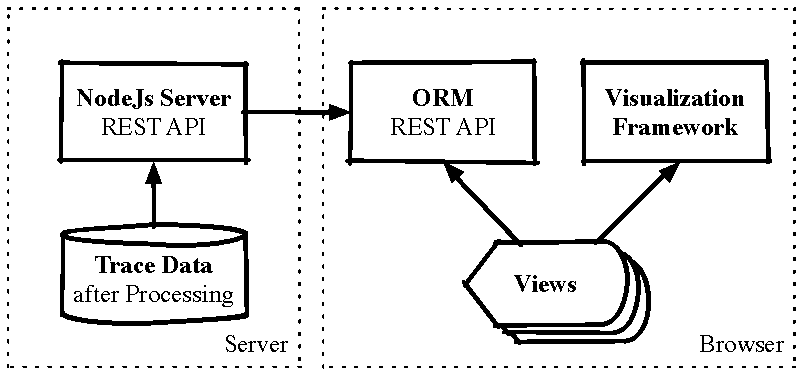
\includegraphics[width=\linewidth]{img/visualization_framework}
\caption{The visualization infrastructure of Parceive.}
\label{fig:visualization}
\end{figure}

\paragraph{Trace Optimization}
As mentioned previously, Parceive uses a database to store trace data. Its
layout is tuned for write operations to reduce the runtime overhead. All the
information required by the views can be obtained via database queries.
However, most of the read operations would take a disproportionate amount of
time to complete without applying certain optimizations on the trace database.
Hence, we perform a set of optimizations during a post-processing step to
reduce lookup times for views.

The most important optimization is the generation of table indices for
efficiently searching the database. Another optimization is the creation of
intermediate tables to avoid expensive joins for most queries. Although this
leads to some redundancy, it does not increase the overall complexity.
Furthermore, reducing fragmentation within tables increases data locality and
thus speeds up queries. This has considerable effect on queries that require a
full table scan and also reduces the size of the trace database.

\paragraph{On-Demand Loading}
On-demand loading of trace data improves responsiveness of the visualization.
Often, loading entire traces into the browser is not feasible due to memory
restrictions. To solve this problem, a NodeJS server has been developed that
reads data on demand. The server provides a REST~\cite{rest} API to manage
retrieval of data. For security reasons, all SQL queries are performed by the
server without supporting arbitrary queries. The implementation makes use of
multiple parallel reads to the database to reduce the latency and to increase
the throughput when large amounts of data are requested by the views. This lets
users seamlessly explore and navigate through software producing a potentially
unmanageable amount of trace data.

\paragraph{Caching and Pipelining}
At the client side, we provide an Object Relational Mapper (ORM) module to
simplify development and improve responsiveness. This module enables accesses
to predefined entities and manages the relationships between them. The API is
implemented using promises~\cite{promises}, which simplify asynchronous and
parallel access. The greatest benefit of views using ORM are optimizations
for data loading, the most important ones being caching and pipelining. Caching
avoids repeated loading of data that was accessed before, and pipelining
combines multiple queries to the same endpoint into a single one. When
requesting a large number of entities, pipelining heavily improves the
throughput with only small latency overhead.

\paragraph{State Management and Communication}
The visualization framework provides global state management and communication
facilities for views. The former is based on a centralized and persistent state
storage that retains the state of views across page loads. Currently,
the view layout and the marked nodes are automatically stored as part of the
state. In addition, each view can save tailored information at any time and
retrieve it during rendering. Local storage is used to keep all the state
information, making it persistent. This service reduces computational effort
for views by reusing results across UI events.

The communication service enables arbitrary views to interact by triggering
predefined events. These events let users explore their applications with
synchronized representations from complementary viewpoints. One example is
simultaneous highlighting of entities such as functions in different views.
Another example is spotting of distinct entities for further inspection in
separate views. This way, the number of nodes to be displayed in a view is
reduced, which increases scalability. Currently the following types of
communication provided:

\begin{itemize}
	\item \textit{Focusing} brings entities to the attention of the user by
centering the representations in all views.
	\item \textit{Marking} allows to share selected entities between views.
	\item \textit{Spotting} replaces the shown entities in views by a new
collection of entities.
	\item \textit{Hovering} highlights entities in multiple views by reducing the
opacity of all other entities.
\end{itemize}

\begin{figure*}[ht!]
	\begin{center}
		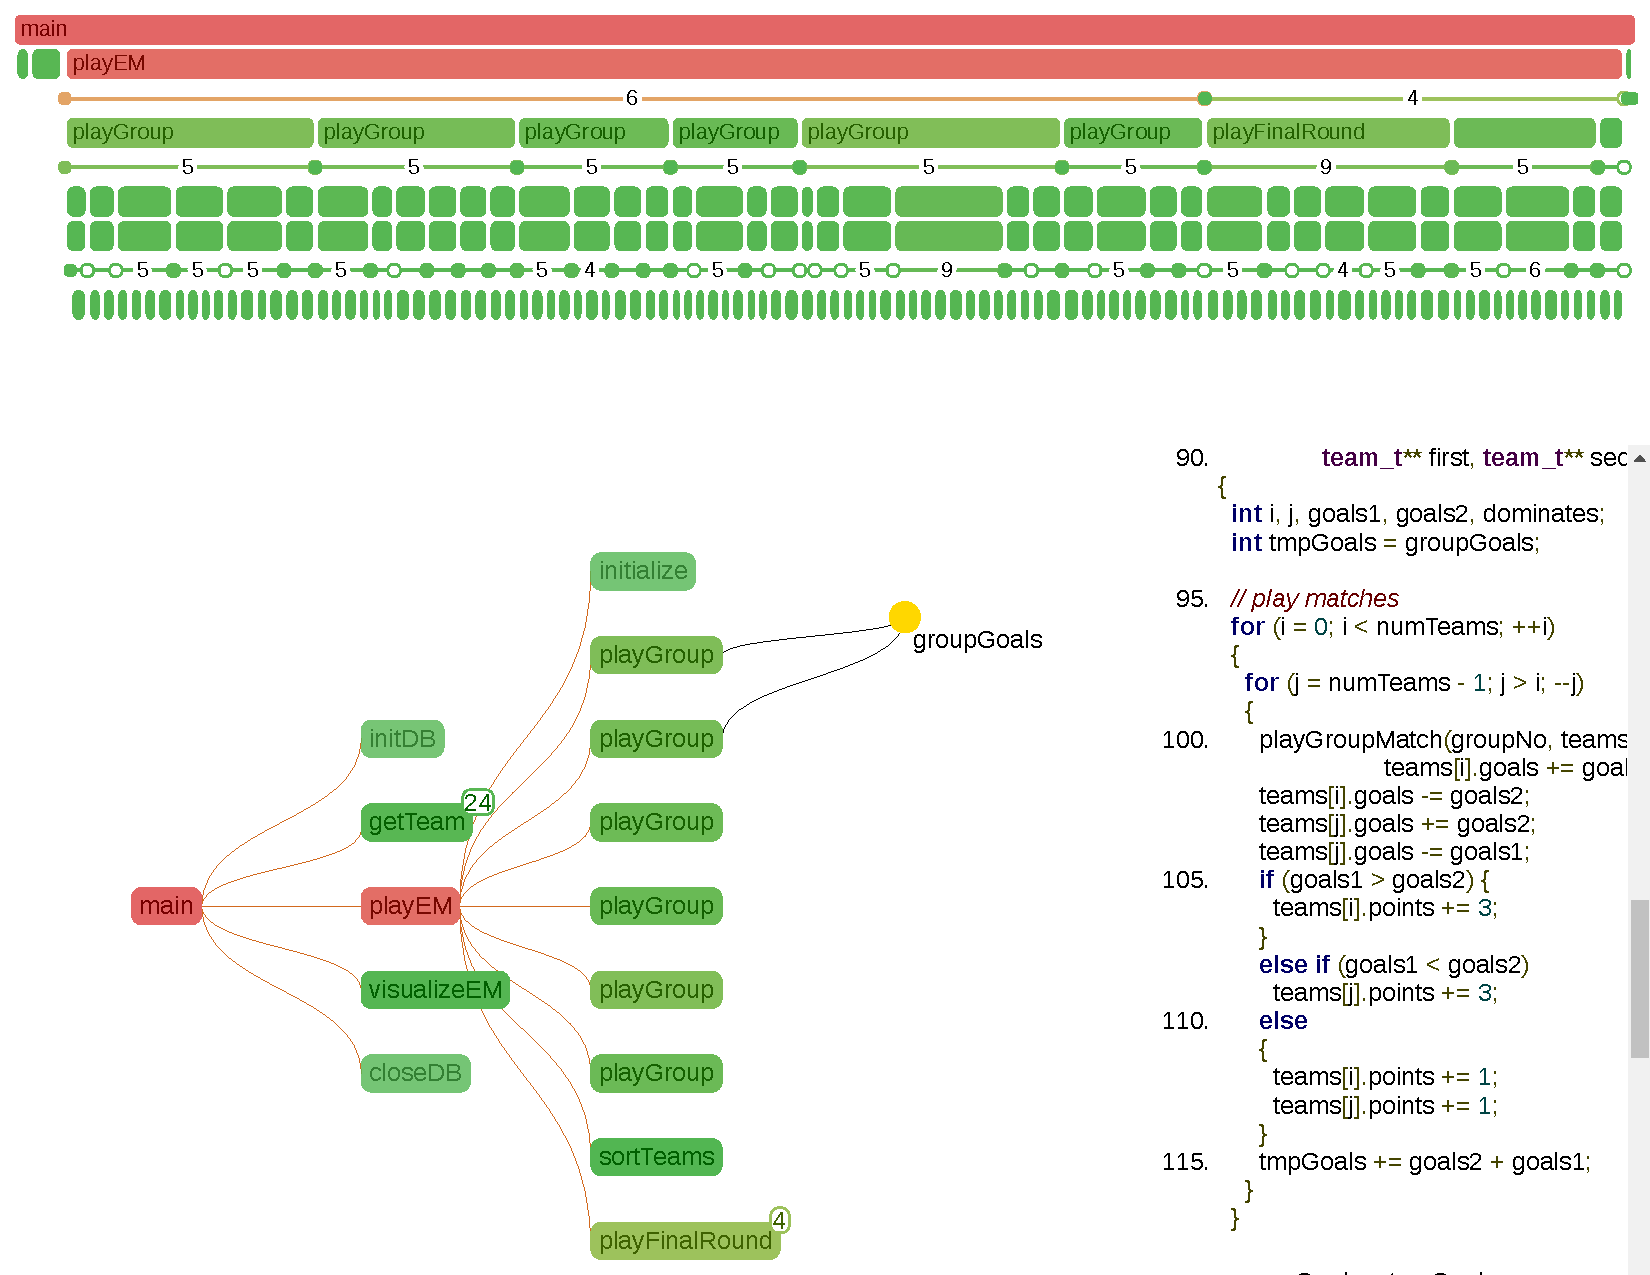
\includegraphics[clip, trim=0.1cm 16.0cm 0.1cm 0.1cm,
width=\linewidth]{img/performance_view.pdf}
		\caption{The performance view of Parceive (trace mode) showing an execution
of EMSim.}
		\label{fig:emsim}
	\end{center}
\end{figure*}